%% ==========================================================================
%%  The Universal Warmup Path
%%  Route-indexed attractors and finite-transcript gates
%% ==========================================================================

\documentclass[11pt]{article}

\usepackage[letterpaper,margin=1.15in]{geometry}
\usepackage{microtype}
\emergencystretch=3em
\usepackage{amsmath,amssymb,amsthm,mathtools}
\usepackage{booktabs}
\usepackage{multirow}
\usepackage{float}
\usepackage{graphicx}
\usepackage{tikz}
\usetikzlibrary{arrows.meta,calc,positioning,shapes.geometric}
\usepackage{listings}
\usepackage{xcolor}
\definecolor{okblue}{HTML}{0072B2}
\definecolor{okvermil}{HTML}{D55E00}
\definecolor{okgreen}{HTML}{009E73}
\definecolor{codegreen}{rgb}{0,0.6,0}
\definecolor{codegray}{rgb}{0.5,0.5,0.5}
\definecolor{codepurple}{rgb}{0.58,0,0.82}
\definecolor{backcolour}{rgb}{0.96,0.96,0.94}
\lstdefinestyle{mystyle}{
  backgroundcolor=\color{backcolour},commentstyle=\color{codegreen},
  keywordstyle=\color{magenta},numberstyle=\tiny\color{codegray},
  stringstyle=\color{codepurple},basicstyle=\ttfamily\footnotesize,
  breaklines=true,captionpos=b,keepspaces=true,numbers=left,
  numbersep=5pt,showspaces=false,showstringspaces=false,tabsize=2}
\lstset{style=mystyle}
\usepackage{natbib}
\bibliographystyle{plainnat}
\usepackage[colorlinks=true,linkcolor=blue!55!black,citecolor=blue!55!black,
            urlcolor=blue!55!black]{hyperref}
\usepackage{authblk}

\theoremstyle{plain}
\newtheorem{theorem}{Theorem}
\newtheorem{lemma}[theorem]{Lemma}
\newtheorem{proposition}[theorem]{Proposition}
\newtheorem{corollary}[theorem]{Corollary}
\theoremstyle{definition}
\newtheorem{definition}[theorem]{Definition}
\theoremstyle{remark}
\newtheorem{remark}[theorem]{Remark}

\newcommand{\Rhat}{\widehat R}
\newcommand{\op}{\mathrm{op}}

\title{\textbf{The Universal Warmup Path:\\[2pt]
Many Routes, One Compass}}
\author{Junpeng Lao}
\date{26 July 2026}

\begin{document}
\maketitle

\begin{abstract}\noindent
Sampler transitions are local, but their efficiency is governed by global
posterior geometry. Warmup bridges the two by tuning the step size, metric, and
related controls. Although these adaptation mechanisms are individually well
studied, their orchestration is still commonly encoded through fixed schedules
and heuristic choices: users preselect the metric family, compute budget, and
response to incompatible geometry. We recast that orchestration as
evidence-based routing within a declared budget. The Universal Warmup Path uses
one sampler-independent compass, $\Sigma_\pi=\operatorname{Cov}_\pi(X)$, while
allowing each route to deploy its own metric. Its discipline---gather evidence,
act, wait, or refuse---is sampler-independent; we evaluate one gradient-based
HMC-family realization using scalar gates. The confidence-aware design gives
route-attractor guarantees, while a finite-transcript bound limits what
confined evidence can establish. When local and global evidence agree, the path
deploys an efficient local metric; disagreement fails loudly through
reparameterization advice or population handoff, never certifying global
coverage. Across the cells we tested, automatic warmup outperformed the
predeclared Fisher low-rank primary, with geometric-mean ESS-per-gradient
ratios of $1.409$--$2.451$ on the ill-conditioned suite and $1.131$--$1.951$ on
German credit. It also improved ESS per gradient over the predeclared
fixed-schedule diagonal control while meeting the same declared post-sampling
quality criterion. The proposed path points toward a coherent theory of sampler
hyperparameter tuning, connecting local adaptation, global geometry, and
explicit refusal in practical controllers.
\end{abstract}

\section{Introduction}\label{sec:intro}

Hamiltonian Monte Carlo (HMC) uses local evaluations of a target to explore a
global distribution \citep{duane1987hybrid,neal2011mcmc}. Its metric and step
size determine whether those local moves resolve the typical set efficiently;
NUTS adapts trajectory length around the same geometry
\citep{hoffman2014nuts}. Warmup must learn that geometry from the least
trustworthy part of the run: correlated trajectories before representativeness
has been established.

This paper treats warmup as a hybrid route-plus-metric dynamical system. Each
estimator branch $a$ has a population functional
\[
  G_a^\star=T_a(\pi).
\]
Examples include diagonal scale, a pooled-within low-rank correction, and a
between-means low-rank correction. The two low-rank branches may share a
reported label while targeting different population objects. The proposed
confidence-aware latch selects a branch only after its confidence set clears
that branch's eligibility region; conditional on a stable route episode, the
population metric map may then attract the iterate to $G_a^\star$.

Four questions remain distinct throughout. \emph{Attraction} asks whether a
fixed route contracts. \emph{Structural identification} asks whether the
transcript resolves a rank or subspace. \emph{Representativeness} asks whether
the transcript has missed important regions. \emph{Utility} asks whether an
identified structure improves compute-adjusted sampling. None implies the next.

The resulting warmup path is universal in a procedural sense: gather evidence,
promote only when the evidence supports a route, and refuse unsupported
geometry. Under a declared constant-metric adequacy criterion, funnels and
scale-coupling targets route to reparameterization. Genuinely regional mixtures
route instead to the companion population/ensemble method over regional
attractors. Refusal is therefore an intended outcome, not a failed metric fit.

Our contributions are a route-indexed attractor theorem with explicit finite-
window error terms; a Markov-transcript uncertainty construction and its
operator consequences; a finite-horizon local-transcript information bound;
and a scalar-gate implementation that keeps identification, consistency, and
utility separate. The controlled Gaussian-mixture study holds the marginal
spectrum fixed while the recorded within/between evidence and route change,
exposing both the value and the limits of the gate. The empirical corpus
separates a predeclared Fisher low-rank primary, a diagonal control, and a
historical shared-step implementation comparison.

Section~\ref{sec:setup} fixes the metric convention, and
Section~\ref{sec:controller} gives the practical route tree.
Sections~\ref{sec:attractor}--\ref{sec:transcript} develop the local guarantees
and limits. Section~\ref{sec:efficiency} reports the empirical comparisons;
implementation, related work, and scope follow, with proofs and supporting
studies in the appendices.

\section{Metric convention and warmup routes}\label{sec:setup}

Let $\pi(x)\propto\exp\{\mathcal L(x)\}$ on $\mathbb R^d$. We use the
\emph{inverse-mass} convention
\begin{equation}
  p\sim\mathcal N(0,G^{-1}),\qquad
  K(p)=\tfrac12p^\top Gp.                                    \label{eq:metric}
\end{equation}
Thus BlackJAX's \texttt{inverse\_mass\_matrix} is $G$. For
$x\sim\mathcal N(\mu,\Sigma)$, Hamilton's equations give
$\ddot x=-G\Sigma^{-1}(x-\mu)$, so the covariance-matching choice is
$G^\star=\Sigma$.

For a general target with finite second moments, define the universal
sampler-independent covariance reference
\[
  \Sigma_\pi=\operatorname{Cov}_\pi(X).
\]
It is a common reference, not a common route estimand: a Fisher, masked,
regularized, or finite-rank route need not target $\Sigma_\pi$.

For a route $a$, let $G_a^\star=T_a(\pi)$ and define the affine-invariant
residual
\[
  R_a(G)=G^{-1/2}G_a^\star G^{-1/2}.
\]
The tangent from $G$ toward $G_a^\star$ is represented by
$\log R_a(G)$ in the whitened frame. This is not interchangeable with the
log-Euclidean difference $\log G_a^\star-\log G$ unless the matrices commute.
For the recursion below we work in a bounded SPD chart $\theta=\log G$; the
route-specific moment-to-metric map is part of $T_a$, not silently identified
with either matrix logarithm.

Classical window adaptation updates step size in fast and slow intervals, while
learning covariance only in expanding, memoryless slow intervals
\citep{carpenter2017stan,cmdstan239warmup}. Fisher-divergence
preconditioning adds a low-rank-plus-diagonal option
\citep{seyboldt2026preconditioning}. Automatic warmup must decide not only how
to estimate within a branch, but when the transcript makes that branch eligible.

\section{Controller and evaluation protocol}\label{sec:controller}

The evaluated implementation starts diagonal and constructs its decision
schedule from dimension $d$, chain count $M$, and total gradient budget
$\mathcal B$. For NUTS it assigns
$\lfloor\mathcal B/(20M)\rfloor$ transitions to each chain, using $20$ as a
conservative gradients-per-transition allowance; a fixed-$L$ kernel uses its
declared integration length in place of $20$. The dimension-derived rank
capacity and pooled support floor are
\[
 k_{\mathrm{cap}}=\min\{50,\max(\lfloor d/2\rfloor,1)\},
 \qquad N_{\min}=8(k_{\mathrm{cap}}+1).
\]
After a harmless one-step initialization window, the first evidence-bearing
window has
$n_1=\lceil N_{\min}/M\rceil$ transitions per chain. Metric windows then have
nominal $1.5\times$ growth. When another grown window would not fit before the
step-size-only phase, the last slow window instead absorbs the remaining metric
transitions. The final $15\%$ adapts step size only. These boundaries are fixed
before sampling begins.

At each prescribed metric-window endpoint, the controller finalizes the
current $M$-chain buffer, recomputes the evidence, and resets the buffer. The
route-specific conjunction combines the W or T structural tests, the
$R^2$ metric-fixability check, and enough remaining budget for the selected
rank and step-size readaptation. A supported W route deploys a low-rank metric
from pooled, per-chain-centered within-chain information. A supported T route
deploys a between-means low-rank correction. Unsupported or inconclusive
evidence leaves the metric diagonal and advances to the next larger scheduled
window. Decisions occur only at endpoints: the evaluated implementation
neither terminates within a window nor moves a boundary in response to the
data.

\begin{figure}[H]\centering
\resizebox{0.98\linewidth}{!}{%
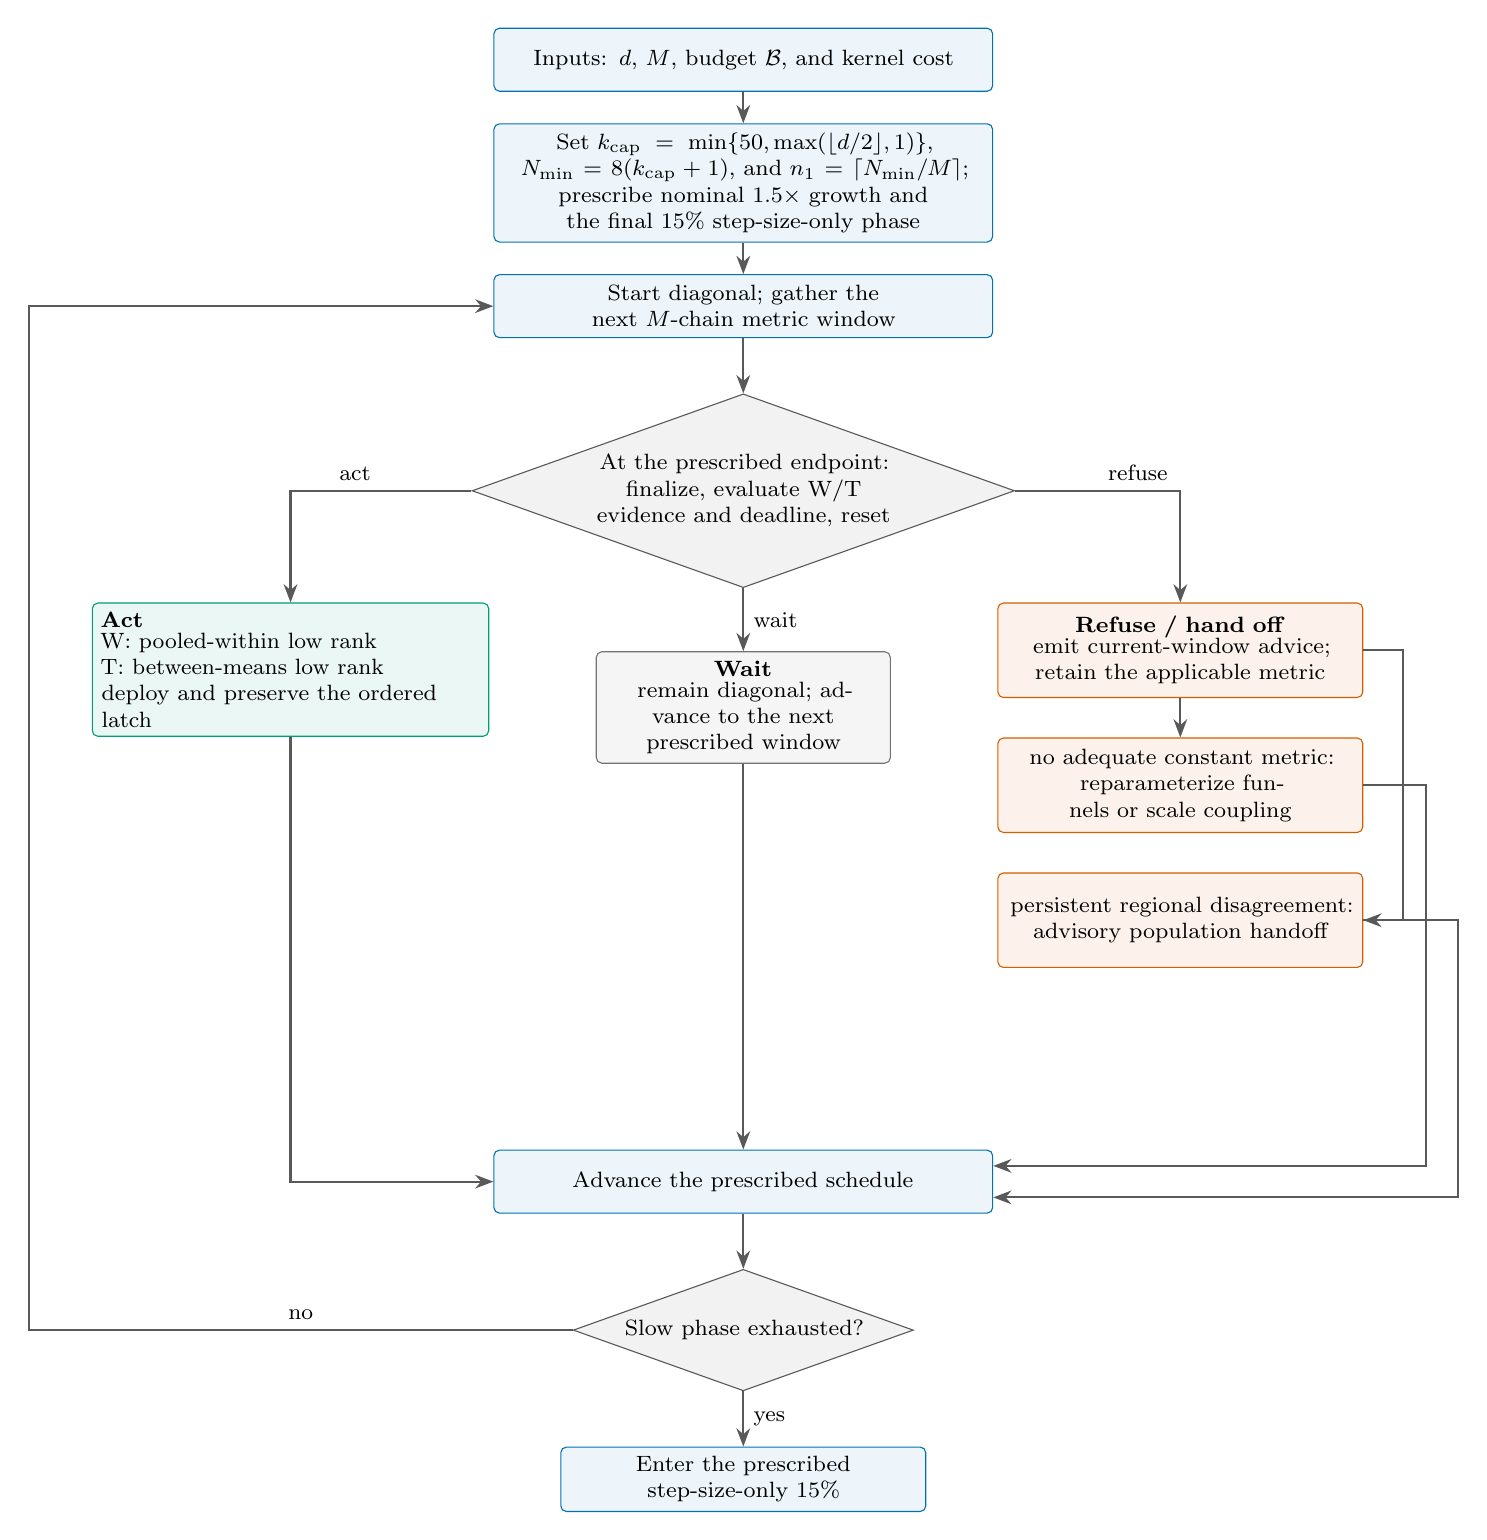
\begin{tikzpicture}[
  font=\footnotesize,
  >=Stealth,
  line/.style={->,thick,draw=black!65},
  proc/.style={draw=okblue,fill=okblue!7,rounded corners=2pt,
               align=center,minimum height=8mm,text width=6.1cm},
  decision/.style={diamond,draw=black!65,fill=black!5,aspect=2.8,
                   align=center,inner sep=1.2pt,text width=4.0cm},
  act/.style={draw=okgreen,fill=okgreen!8,rounded corners=2pt,
              align=left,minimum height=13mm,text width=4.8cm},
  wait/.style={draw=black!55,fill=black!4,rounded corners=2pt,
               align=center,minimum height=13mm,text width=3.5cm},
  refuse/.style={draw=okvermil,fill=okvermil!8,rounded corners=2pt,
                 align=center,minimum height=12mm,text width=4.4cm},
  final/.style={draw=okblue,fill=okblue!7,rounded corners=2pt,
                align=center,minimum height=8mm,text width=4.4cm}
]
\node[proc] (inputs) {Inputs: $d$, $M$, budget $\mathcal B$, and kernel cost};
\node[proc,below=4mm of inputs] (schedule) {Set
  $k_{\rm cap}=\min\{50,\max(\lfloor d/2\rfloor,1)\}$,
  $N_{\min}=8(k_{\rm cap}+1)$, and
  $n_1=\lceil N_{\min}/M\rceil$; prescribe nominal $1.5\times$ growth and the
  final $15\%$ step-size-only phase};
\node[proc,below=4mm of schedule] (gather) {Start diagonal; gather the next
  $M$-chain metric window};
\node[decision,below=7mm of gather] (boundary) {At the prescribed endpoint:
  finalize, evaluate W/T evidence and deadline, reset};
\node[act,below left=8mm and 15mm of boundary] (act) {
  \textbf{Act}\\[-2pt]
  W: pooled-within low rank\\
  T: between-means low rank\\
  deploy and preserve the ordered latch};
\node[wait,below=8mm of boundary] (wait) {
  \textbf{Wait}\\[-2pt]
  remain diagonal; advance to the next prescribed window};
\node[refuse,below right=8mm and 15mm of boundary] (refuse) {
  \textbf{Refuse / hand off}\\[-2pt]
  emit current-window advice; retain the applicable metric};
\node[refuse,below=5mm of refuse,text width=4.4cm] (reparam) {
  no adequate constant metric:\\ reparameterize funnels or scale coupling};
\node[refuse,below=5mm of reparam,text width=4.4cm] (population) {
  persistent regional disagreement:\\ advisory population handoff};
\node[proc,below=49mm of wait] (continue) {Advance the prescribed schedule};
\node[decision,below=7mm of continue,text width=3.3cm] (exhausted)
  {Slow phase exhausted?};
\node[final,below=7mm of exhausted] (final) {Enter the prescribed
  step-size-only $15\%$};
\coordinate (looplow) at ([xshift=-8mm]act.west |- exhausted.west);
\coordinate (loopup) at ([xshift=-8mm]act.west |- gather.west);

\draw[line] (inputs) -- (schedule);
\draw[line] (schedule) -- (gather);
\draw[line] (gather) -- (boundary);
\draw[line] (boundary) -| node[pos=0.25,above left]{act} (act);
\draw[line] (boundary) -- node[right]{wait} (wait);
\draw[line] (boundary) -| node[pos=0.25,above right]{refuse} (refuse);
\draw[line] (refuse) -- (reparam);
\draw[line] (refuse.east) -- ++(5mm,0) |- (population.east);
\draw[line] (act.south) |- (continue.west);
\draw[line] (wait.south) -- (continue.north);
\draw[line] (reparam.east) -- ++(8mm,0) |- ([yshift=2mm]continue.east);
\draw[line] (population.east) -- ++(12mm,0) |- ([yshift=-2mm]continue.east);
\draw[line] (continue) -- (exhausted);
\draw[line] (exhausted) -- node[right]{yes} (final);
\draw[line] (exhausted.west) -- node[above]{no} (looplow)
  -- (loopup) -- (gather.west);
\end{tikzpicture}%
}
\caption{The evaluated warmup path. Setup fixes every window boundary before
execution, and evidence is evaluated only at metric-window endpoints. Every
outcome continues the prescribed scan: acting preserves the selected route,
waiting advances while diagonal to the next prescribed window, and the two advisory
leaves retain the applicable metric. Only exhaustion of the metric-adapting
phase enters the final step-size-only $15\%$. This is not an early-stopping or
change-point rule.}
\label{fig:warmup-path}
\end{figure}

Persistent regional disagreement can coexist with a W-selected,
within-chain-conditioned metric. It produces a current-window advisory handoff
to the companion population/regional ensemble; it never establishes global
exploration, which is reported as \texttt{not\_established}. Reparameterization
is a separate no-adequate-constant-metric route. Both advisory outputs are
recomputed at later endpoints and may clear while the scan continues. A
companion local-trajectory
sampler may consume the selected local metric, while the population method owns
discovery, exchange, and weighting across regional attractors. The theorem-level
design below promotes only after confidence-ball inclusion; the evaluated
implementation realizes the same act--wait--refuse discipline with scalar
gates, not with those confidence objects.

Estimator, window schedule, metric-buffer policy, and step-size controller are
independent engineering choices. The Fisher-HMC reference prescription in this
paper is specifically the $30/55/15$ schedule of
\citet{seyboldt2026preconditioning}: it uses $L=10$ and then $L=80$
refresh/memory periods, periodically wipes older draws, and reinitializes step
size once at the start of phase 2. It is not a generic description of every
\texttt{nutpie} version. Stan's expanding slow windows are successively doubled
in the version 2.39 CmdStan User's Guide \citep{cmdstan239warmup}.

The empirical schedule evidence compares configuration bundles and does not
isolate the causal effect of window shape; its limited reseed ablation does not
establish Stan--nutpie equivalence. Figure~\ref{fig:schedule} in
Appendix~\ref{app:schedule} records the schedule prescriptions and one
executed trace.

\section{Route-indexed attractor dynamics}\label{sec:attractor}

Let $\eta_k$ be the target-population routing object at the current metric,
including the population moments and whitening transformation declared by the
candidate route. Let $C_k$ be its confidence set at the end of window $k$ and
$H_b$ the eligibility region for promotion to route $b$. Coverage of $C_k$ must
pay for starting-law, within-window adaptation, whitening, sampling, and
regularization errors. Routes form an ordered, one-transition latch: once
promoted, the controller does not demote during that route episode.

\begin{lemma}[Simultaneous soundness of the confidence-aware latch]\label{lem:latch}
Let $\mathcal K$ be the fixed, declared set of potential decision windows.
Suppose
\[
  \Pr(\eta_k\notin C_k\mid\mathcal F_{k-1})\le\delta_k
\]
for every $k\in\mathcal K$, whether or not a promotion is ultimately attempted.
Promote to $b$ only when $C_k\subset H_b$. Then, with probability at least
$1-\sum_{k\in\mathcal K}\delta_k$, every promotion made by the latch is
supported by the true routing estimand at the time of promotion.
\end{lemma}

The lemma certifies only the declared target-population estimand at the
promotion time. Persistent optimality and global target coverage require
separate arguments. A fixed-window Wald set is not automatically a valid
repeated-use sequence; a deployed sequential latch needs confidence spending
or an anytime-valid construction.

After promotion, consider a route episode on branch $a$. Let $s(\theta)$ be its
population routing statistic, $g$ the router, $h_a(\theta)$ the population
update field, and $\theta_a^\star=\log G_a^\star$. Write
\begin{equation}
  F_a(\theta)=\theta+\alpha h_a(\theta),\qquad
  \theta_{k+1}=\widehat F_{k,a}(\theta_k).                    \label{eq:update}
\end{equation}

\begin{theorem}[Local robust attractor of a route episode]\label{thm:attractor}
Let $\Theta$ be the bounded log-SPD chart used by the controller. Assume
$R_0>0$, $\theta_a^\star\in\Theta$, and
$\overline B_F(\theta_a^\star,R_0)\subset\Theta$, where
$\overline B_F$ denotes a closed Frobenius-norm ball. Assume also that
$s(\theta_a^\star)\in\operatorname{int}(\mathcal S_a)$, where
$\mathcal S_a=\{s:g(s)=a\}$. Suppose $h_a(\theta_a^\star)=0$ and, on
$\overline B_F(\theta_a^\star,R_0)$, for constants $\mu>0$ and $L_h>0$,
\[
 \langle\theta-\theta_a^\star,h_a(\theta)\rangle_F
 \le-\mu\|\theta-\theta_a^\star\|_F^2,\qquad
 \|h_a(\theta)\|_F\le L_h\|\theta-\theta_a^\star\|_F.
\]
Let $0<\alpha<2\mu/L_h^2$ and
$q=(1-2\alpha\mu+\alpha^2L_h^2)^{1/2}<1$. For every $k<K$, suppose
candidate statistics and updates are constructed before routing, and define
the joint error event
\[
\begin{aligned}
\mathcal E_k={}&
 \{\|\widehat s_k-s(\theta_k)\|_{\mathcal S}>r_k^s\}\\
 &{}\cup
 \{\|\widehat F_{k,a}(\theta_k)-F_a(\theta_k)\|_F>e_k\},
 \qquad
 \Pr(\mathcal E_k\mid\mathcal F_{k-1})\le\delta_k .
\end{aligned}
\]
Here $\|\cdot\|_{\mathcal S}$ is the declared statistic-space norm. Let $s$ be
$L_s$-Lipschitz from the ball to that norm, let
$\kappa=\operatorname{dist}\{s(\theta_a^\star),
\partial\mathcal S_a\}>0$, with distance in the same norm. Subject to the
ordered latch, the observable rule selects or promotes candidate branch $a$
whenever the following inclusion holds, and otherwise abstains:
\[
\overline B_{\mathcal S}(\widehat s_k,r_k^s)\subset\mathcal S_a.
\]
For every $k<K$, assume $L_sR_0+2r_k^s<\kappa$ and
$e_k\le(1-q)R_0$; the derived margin is sufficient for the observable
inclusion on the good event.
If $\|\theta_0-\theta_a^\star\|_F\le R_0$ and the latch is unset or already
correctly set to $a$, then on the simultaneous good event the router selects
$a$, the iterates remain in the ball, and
\begin{equation}
 \|\theta_K-\theta_a^\star\|_F
 \le q^K\|\theta_0-\theta_a^\star\|_F
     +\sum_{j=0}^{K-1}q^{K-1-j}e_j.                          \label{eq:contract}
\end{equation}
This event has probability at least $1-\sum_{k<K}\delta_k$.
\end{theorem}

The finite-window update-error budget is deliberately explicit:
\begin{equation}
 e_k\le e_k^{\rm start}+e_k^{\rm step}+e_k^{\rm white}
          +e_k^{\rm sample}+e_k^{\rm reg}.                   \label{eq:errors}
\end{equation}
These terms cover the starting law, adaptive step size, estimated whitening,
sampling fluctuation, and regularization. Controlled-Markov stability,
convergence, and ergodicity results provide asymptotic ingredients under
conditions such as drift, containment, and diminishing adaptation; they do not
themselves provide route-specific finite-window high-probability bounds for
$e_k^{\rm start}$ or $e_k^{\rm step}$. Invariant kernels alone do not remove
transient or state-dependent adaptation bias
\citep{andrieu2005stability,fort2016convergence,roberts2007coupling}.
The scalar-gate implementation has not calibrated or verified the five
component bounds in \eqref{eq:errors}. The theorem applies once those
route-specific bounds have been established.

\section{Uncertainty and safe structural gates}\label{sec:ident}

\subsection{Universal covariance and route identification}\label{sec:covbridge}

For $M$ equal-length chains with $n$ recorded states, write $\bar x_m$ for
chain $m$'s mean and $\bar x$ for the grand mean, and define
\[
 W=\frac{1}{M(n-1)}\sum_{m=1}^M\sum_{t=1}^n
 (x_{mt}-\bar x_m)(x_{mt}-\bar x_m)^\top,
\]
\[
 B=\frac{n}{M-1}\sum_{m=1}^M
 (\bar x_m-\bar x)(\bar x_m-\bar x)^\top.
\]
If $S$ is the ordinary covariance of all $Mn$ states about $\bar x$, then
\begin{equation}
 (Mn-1)S=M(n-1)W+(M-1)B.                                  \label{eq:anova}
\end{equation}
This finite-transcript identity is exact: it requires neither independence nor
stationarity. It remains exact after one common realized linear projection
$A$, with $S,W,B$ replaced by $ASA^\top,AWA^\top,ABA^\top$. A projection
selected from the same data is still algebraically descriptive, but calibrated
post-selection inference requires cross-fitting, selective inference, or a
simultaneous operator bound. Separately whitening $S$, $W$, and $B$ does not
preserve \eqref{eq:anova}.

Now hold $M$ fixed and let $n\to\infty$. Suppose each chain's empirical first
and second moments converge to those of a law $\nu_m$. Then $S$ converges to
the covariance of the equal aggregate mixture
\[
 \bar\nu=\frac1M\sum_{m=1}^M\nu_m.
\]
This limit identifies $\Sigma_\pi$ only when $\bar\nu$ is second-moment
representative of $\pi$. Agreement among chains is not enough: a clean ensemble
confined to one basin can converge to the wrong regional covariance.

\begin{figure}[H]\centering
\resizebox{0.98\linewidth}{!}{%
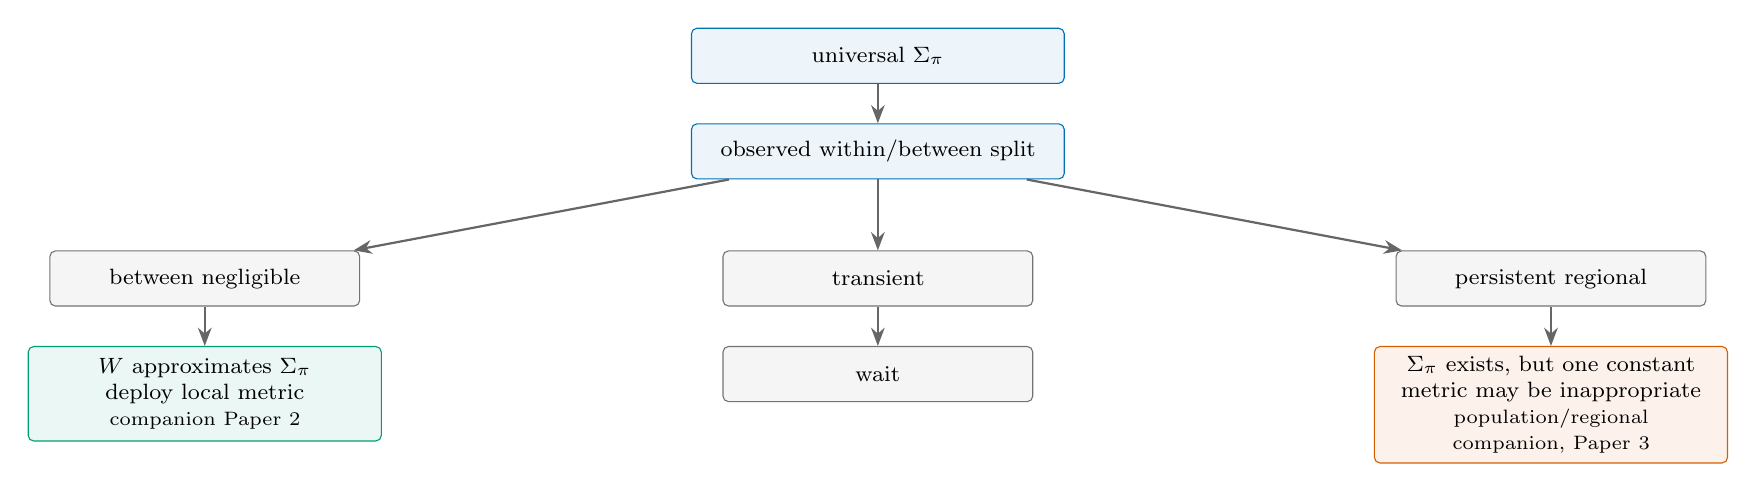
\begin{tikzpicture}[
  font=\footnotesize,
  >=Stealth,
  edge/.style={->,thick,draw=black!60},
  root/.style={draw=okblue,fill=okblue!7,rounded corners=2pt,
               align=center,minimum height=7mm,text width=4.5cm},
  branch/.style={draw=black!55,fill=black!4,rounded corners=2pt,
                 align=center,minimum height=7mm,text width=3.7cm},
  local/.style={draw=okgreen,fill=okgreen!8,rounded corners=2pt,
                align=center,minimum height=12mm,text width=4.25cm},
  regional/.style={draw=okvermil,fill=okvermil!8,rounded corners=2pt,
                   align=center,minimum height=12mm,text width=4.25cm}
]
\node[root] (sigma) {universal $\Sigma_\pi$};
\node[root,below=5mm of sigma] (split) {observed within/between split};
\node[branch,below left=9mm and 42mm of split] (negligible)
  {between negligible};
\node[branch,below=9mm of split] (transient) {transient};
\node[branch,below right=9mm and 42mm of split] (persistent)
  {persistent regional};
\node[local,below=5mm of negligible] (deploy)
  {$W$ approximates $\Sigma_\pi$\\deploy local metric\\{\scriptsize companion Paper 2}};
\node[branch,below=5mm of transient] (wait) {wait};
\node[regional,below=5mm of persistent] (ensemble)
  {$\Sigma_\pi$ exists, but one constant metric may be inappropriate\\
   {\scriptsize population/regional companion, Paper 3}};

\draw[edge] (sigma) -- (split);
\draw[edge] (split) -- (negligible);
\draw[edge] (split) -- (transient);
\draw[edge] (split) -- (persistent);
\draw[edge] (negligible) -- (deploy);
\draw[edge] (transient) -- (wait);
\draw[edge] (persistent) -- (ensemble);
\end{tikzpicture}%
}
\caption{Practical interpretation of the universal covariance reference through
the observed within/between split. The leaves scope metric use and the next
method; they do not certify discovery or coverage of unseen regions.}
\label{fig:covariance-tree}
\end{figure}

\begin{proposition}[When covariance identifies a route]\label{prop:fibre}
Let $\mathcal P$ be a declared target class with finite covariance. A route
functional $T_a$ is identified by covariance on $\mathcal P$ if and only if it
is constant on covariance fibres:
\[
 \operatorname{Cov}_{\pi_0}(X)=\operatorname{Cov}_{\pi_1}(X)
 \quad\Longrightarrow\quad T_a(\pi_0)=T_a(\pi_1)
 \qquad(\pi_0,\pi_1\in\mathcal P).
\]
Equivalently, there is a map $F_a$ on the covariance range of $\mathcal P$ such
that $T_a(\pi)=F_a(\Sigma_\pi)$. This condition preserves the route-indexed
target $G_a^\star=T_a(\pi)$ rather than replacing it by a universal metric.
\end{proposition}

The Fisher route gives a useful full-rank special case. Let
$s(x)=\nabla\log\pi(x)$ and
$J_\pi=E_\pi\{s(X)s(X)^\top\}$.

\begin{proposition}[Full-rank Fisher covariance bound]\label{prop:fisher}
Suppose $\pi$ has a smooth positive density, finite SPD covariance
$\Sigma_\pi$, square-integrable score, and Stein boundary conditions. Then
\[
 E_\pi\{(X-\mu)s(X)^\top\}=-I,\qquad
 J_\pi\succeq\Sigma_\pi^{-1}.
\]
For the unregularized, no-cutoff, full-rank affine-invariant Fisher population
functional, with $\#$ denoting the SPD geometric mean,
\[
 G_F=\Sigma_\pi\#J_\pi^{-1},\qquad
 \Sigma_\pi^{-1/2}G_F\Sigma_\pi^{-1/2}
 =(\Sigma_\pi^{1/2}J_\pi\Sigma_\pi^{1/2})^{-1/2}\preceq I.
\]
Equality holds precisely in the affine-score, hence Gaussian, case under these
assumptions \citep{dembo1991information}.
\end{proposition}

This proposition does not identify the deployed finite-rank, masked,
regularized Fisher route from covariance. For example, a standard Gaussian and
a variance-one Student-$t_\nu$ law have the same covariance, whereas their
one-dimensional location Fisher informations are respectively $1$ and
$\nu(\nu+1)/\{(\nu-2)(\nu+3)\}>1$ for $\nu>2$. Their full-rank Fisher
functionals therefore differ.

\subsection{A route-specific Markov central limit theorem}

For route $a$, collect the quadratic and score observables actually used by
that branch in a vector $f_a(X_t)$, with mean $\eta_a$. For a stationary,
geometrically ergodic frozen-kernel chain with sufficient moments, the
multivariate Markov-chain CLT gives
\begin{equation}
 \sqrt n(\widehat\eta_a-\eta_a)
 \Rightarrow\mathcal N(0,\Omega_a),\qquad
 \Omega_a=\sum_{h=-\infty}^{\infty}
 \operatorname{Cov}_\pi\{f_a(X_0),f_a(X_h)\}.                 \label{eq:mclt}
\end{equation}
The full long-run covariance (LRV) depends on the functionals in $f_a$; a
single scalar ESS cannot be substituted into an iid Wishart law
\citep{jones2004markov,vats2018strong}.
If $\phi_a$ maps moments to a symmetric residual, let $J_a$ be the derivative
of $\operatorname{vech}\circ\phi_a$ and let
\[
 u=\operatorname{vech}(\widehat R_a-R_a),
\]
where $\operatorname{vech}$ retains one copy of each off-diagonal. The delta
method gives root-$n$ limit covariance
$\Gamma_a=J_a\Omega_aJ_a^\top$ for $\sqrt n\,u$. Let $Q$ be the oracle
population support: its orthonormal columns span
$\operatorname{range}(\Gamma_a)$. Set $z=Q^\top u$ and require
$p=\operatorname{rank}(\Gamma_a)\ge1$. If $\Gamma_a$ is singular, assume
$(I-QQ^\top)u=o_p(n^{-1/2})$, or that the residual lies exactly on the declared
support. Require
$Q^\top\widehat\Gamma_aQ$ to be positive definite and consistent on this
support. For one fixed window, an illustrative Wald construction is
\begin{equation}
 r_{\alpha,n}=
 \left\{\frac{2\chi^2_{p,1-\alpha}
 \lambda_{\max}(Q^\top\widehat\Gamma_aQ)}{n}\right\}^{1/2}.   \label{eq:radius}
\end{equation}
Indeed, for symmetric $A$,
$\|A\|_F\le\sqrt{2}\|\operatorname{vech}(A)\|_2$, which accounts
for the factor $2$ inside the squared radius and yields a Frobenius, hence
operator, radius asymptotically. The construction requires a consistent
multivariate LRV estimator and regularity for the route map. Estimating $Q$ or
its rank from the same window requires a separate justification. With $M$
independent frozen chains, their contributions may scale as $1/M$; chains
coupled through shared adaptation are not automatically independent.
Non-asymptotic matrix concentration is another route only under explicit
boundedness, tail, and dependence assumptions \citep{neeman2024concentration}.

\begin{theorem}[Consequences of an operator-confidence event]\label{thm:operator}
Let $R_a$ and $\widehat R_a$ be symmetric population and estimated residuals,
with eigenvalues in descending order, and suppose
$\|\widehat R_a-R_a\|_{\op}\le r$.
\begin{enumerate}
\item Weyl's inequality gives
  $|\widehat\lambda_j-\lambda_j|\le r$ for every $j$.
\item For a declared population cutoff $\tau$ and $1\le k<d$, if
  $\widehat\lambda_k-r>\tau$ and
  $\widehat\lambda_{k+1}+r<\tau$, then exactly $k$ population eigenvalues
  exceed $\tau$. Otherwise this interval gate abstains.
\item Let $V$ and $\widehat V$ span the matched population and estimated top-$k$
  eigenspaces (or a declared isolated eigenvalue cluster), and let $\Delta$ be
  the minimum population separation between that cluster and its complement.
  If $\Delta>2r$, then
  $\|\sin\Theta(\widehat V,V)\|_{\op}\le2r/\Delta$.
\item If $\lambda_{\min}(R_a)\ge m>r$, then
  \[
    \|\log\widehat R_a-\log R_a\|_{\op}
       \le \log\!\left(\frac m{m-r}\right)\le\frac r{m-r}.
  \]
\end{enumerate}
A metric-error claim additionally requires a route-specific perturbation bound
for the moment-to-metric map $T_a$.
\end{theorem}

These are standard operator, subspace, and SPD-log consequences
\citep{bhatia1997matrix,yu2015useful,higham2008functions}. They show exactly
which margins a confidence-aware gate needs. The deployed cosine statistic
$\Psi$ is a deterministic agreement check between replicated directions:
high agreement is compatible with shared whitening bias and does not establish
accuracy or coverage.

\subsection{The restricted role of BBP calibration}

For iid Gaussian observations from the spiked covariance model with aspect
ratio $\gamma=d/n$, a population spike separates when
$\ell>1+\sqrt\gamma$, while the null sample-noise edge is
$(1+\sqrt\gamma)^2$ \citep{baik2005phase,baik2006eigenvalues,paul2007asymptotics}.
This asymptotic PCA calculation is a useful scale calibration. It is not an
exact edge for Markov draws, a finite-sample if-and-only-if statement, or an
unrestricted information limit. In particular, subthreshold alternatives can
retain nontrivial testing power \citep{onatski2013asymptotic}.

\begin{figure}[H]\centering
  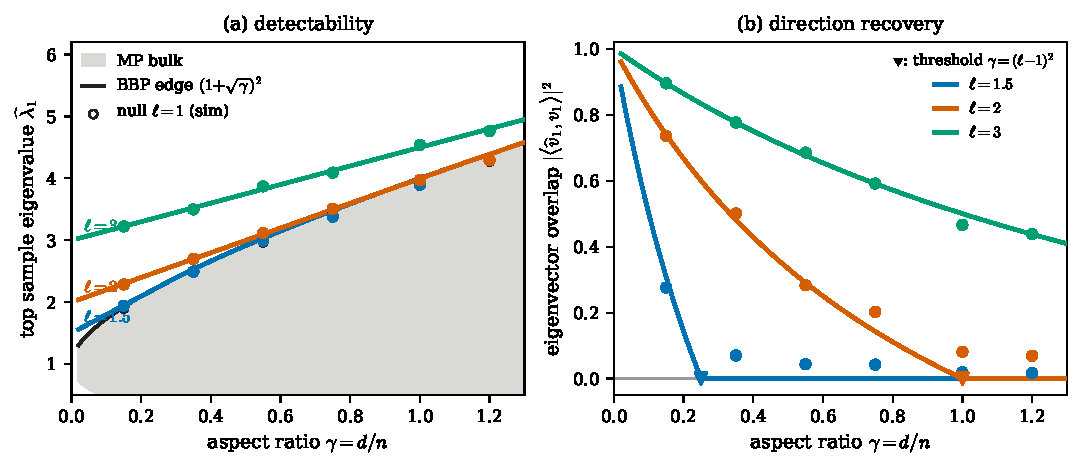
\includegraphics[width=\linewidth]{figures/figure_bbp.pdf}
  \caption{Iid Gaussian spiked-PCA calibration ($d=200$). The curves show the
  asymptotic sample eigenvalue and eigenvector overlap; markers are fixed-seed
  simulations. The population threshold is $1+\sqrt\gamma$, and the null sample
  edge is $(1+\sqrt\gamma)^2$. The figure is not a Markov-chain gate.}
  \label{fig:bbp}
\end{figure}

\subsection{Controlled GMM at fixed marginal geometry}

The controlled target is a five-dimensional, two-component Gaussian mixture
with weights $\pi_1=0.30$, $\pi_2=0.70$,
$v=(1,1,0,0,0)^\top/\sqrt2$, and $a=21$. Its means and shared component
covariance are
\[
 \mu_1=-\pi_2\delta v,\qquad \mu_2=\pi_1\delta v,\qquad
 \Sigma_w=I_5+\beta vv^\top,
\]
where
\[
 \delta^2(\mathrm{SR})
 =\frac{\mathrm{SR}^2(1+a)}{1+\pi_1\pi_2\mathrm{SR}^2},
 \qquad \beta=a-\pi_1\pi_2\delta^2.
\]
Thus
$\Sigma_{\rm marginal}=\Sigma_w+
\pi_1\pi_2(\mu_2-\mu_1)(\mu_2-\mu_1)^\top=I_5+avv^\top$,
so the marginal diagonal-whitened top eigenvalue is $1.913$ throughout the
separation sweep. Separation is indexed by
$\mathrm{SR}=\delta/s(\delta)$, where $\delta$ is the distance between component
means and $s(\delta)=\{v^\top\Sigma_wv\}^{1/2}$ is the within-component standard
deviation along the separation direction $v$. Equation~\eqref{eq:anova}
therefore gives an exact finite-transcript partition for this target. With
latent component labels, the usual within-component plus label-mean-scatter
identity gives the corresponding population partition.

The current sweep keeps the marginal spike fixed at $1.913$ while the
recorded within/between evidence changes. Low-rank routing increasingly gives
way to diagonal routing and an advisory population handoff. The route boundary
is therefore not explained by a changing marginal spectrum, but the recorded
summaries do not isolate a unique occupation mechanism. The handoff is
recomputed from the current window and is non-monotone; it is neither a latch
nor evidence of persistent global exploration. In every row,
\texttt{global\_exploration} remains \texttt{not\_established}.

Compute changes when the disagreement becomes visible: the median onset is
$5.0$ at $20{,}000$, $6.0$ at $60{,}000$, and $7.0$ at $120{,}000$ warmup
gradients. Appendix~\ref{app:gmm-boundary} gives every current $60$k row, the
single-chain contrast, and the matched ablations.

\begin{figure}[H]\centering
  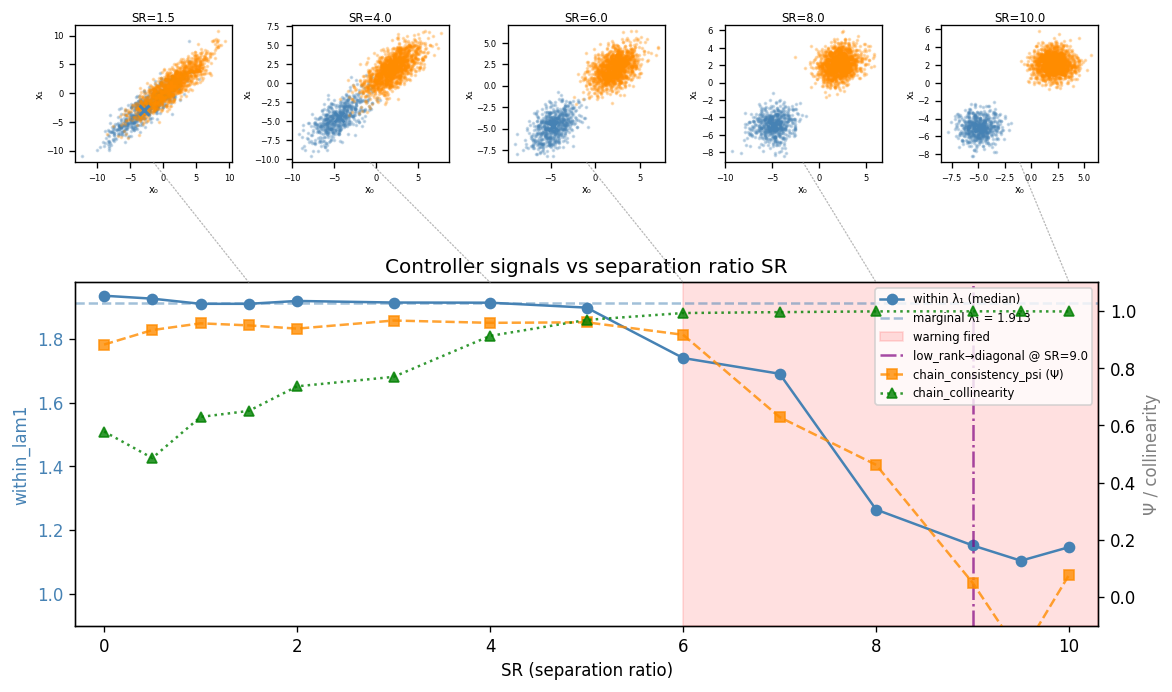
\includegraphics[width=\linewidth]{figures/gmm_money_panel.png}
  \caption{Current-corpus controlled GMM boundary, generated from the current
  $k=2$ primary corpus. Top: target draws at selected separation ratios. Bottom:
  seed-median current diagnostics. The marginal spike remains $1.913$; the
  shading begins at the first grid point with a persistent disagreement signal
  in any seed, and the dash-dot line marks the first all-diagonal grid point.
  These are current-window signals: a population handoff can clear, and
  \texttt{global\_exploration} remains \texttt{not\_established}.}
  \label{fig:gmm-boundary}
\end{figure}

\section{Finite-horizon local transcripts}\label{sec:transcript}

Structural evidence from visited states cannot by itself certify unseen regions.
The appropriate obstruction is finite-horizon and depends on the joint event
that every query remains local.

\begin{theorem}[Local-transcript indistinguishability]\label{thm:transcript}
Let $q_0,q_1$ be smooth, positive, integrable unnormalized targets. Target
access is only through a declared oracle, and the two targets give identical
oracle responses on an open region $A$. Run the same randomized algorithm
through a fixed horizon $T$ from the same initial law under both targets,
couple all random numbers, and assume it makes finitely many oracle calls
almost surely through $T$. Let $E_T$ be the event that every oracle query made
by the complete, possibly interacting algorithm through $T$ lies in $A$.
Induction over oracle queries then gives identical coupled transcripts on
$E_T$ and a common submeasure of mass
\[
 p_T=P_0(E_T)=P_1(E_T).
\]
If the normalized targets $\pi_0,\pi_1$ have metric functionals satisfying
$d\{T(\pi_0),T(\pi_1)\}>2\epsilon$, then every common
transcript-measurable estimator $\widehat T$ satisfies
\begin{equation}
 \Pr_0\{d(\widehat T,T(\pi_0))>\epsilon\}
 +\Pr_1\{d(\widehat T,T(\pi_1))>\epsilon\}\ge p_T.            \label{eq:local}
\end{equation}
Consequently the two-point minimax error is at least $p_T/2$.
\end{theorem}

For replica events $E_{T,m}$, the chain rule is
\[
 p_T=\prod_{m=1}^M
 P(E_{T,m}\mid E_{T,1}\cap\cdots\cap E_{T,m-1}).
\]
Independent replicas give $p_T=\prod_m q_{T,m}$. If every displayed
conditional probability is bounded below by $q_T$, then
$p_T\ge q_T^M$. Identical independent replicas are sufficient for
$p_T=q_T^M$ when each has confinement probability $q_T$, but they are not
necessary: equality in the displayed lower bound occurs whenever every
conditional factor equals $q_T$, including some dependent constructions.
Shared adaptation keeps the joint $p_T$ form. The lower bound applies when
$M=1$ and makes multiple chains neither mathematically necessary nor
sufficient for discrimination. Genuinely overdispersed multiple chains remain
a principal practical safeguard against metastability and unvisited modes.
Longer runs, more starts, or a more diverse collection of starts can reduce the
confinement event, but need not do so at fixed compute.
No fixed sample count is privileged: its meaning is target-, kernel-, start-,
and controller-specific unless $p_T$ is bounded for a declared problem class.
This is a finite-horizon Le Cam two-point coupling argument
\citep{yu1997assouad}.

\section{Routing and efficiency evidence}\label{sec:efficiency}

The scalar-gate implementation selected low rank in all $12/12$
ill-conditioned and German-credit cells. Across automatic, Fisher, and
diagonal arms, all $36/36$ post-sampling population-quality checks passed:
rank-normalized split-$\Rhat$ was finite with maximum at most $1.01$, and
sampling divergences were zero. This is a reporting rule for the observed
population, not routing confidence or a global-exploration result. The corpus
uses ArviZ rank-normalized split-$\Rhat$ \citep{vehtari2021rank}; $4{,}996$
warmup divergences are retained rather than screened from the record.

Table~\ref{tab:eff} compares automatic warmup with the predeclared Fisher
low-rank primary and, separately, the diagonal control. Automatic warmup beats
the Fisher primary in every observed cell under all three ESS-per-gradient
estimands. Every ratio charges gradients actually consumed. The pooled and
marginal fixed-suite comparisons use $M=8$ chains, float64 arithmetic, explicit
integer seeds, and a $312$-transition equal-split population comparator under
the preregistered nominal allocation. Pooled accounting charges all warmup and
sampling gradients; marginal accounting charges one chain's sampling gradients
and $1/M$ of joint warmup, and its geometric means aggregate paired
seed-by-chain ratios. The one-output column is descriptive: its comparator is
the historical single-chain $2{,}500$-warmup policy and is not budget-identical.

\begin{table}[H]\centering
\caption{Geometric-mean automatic/comparator ESS-per-gradient ratios under the
column-specific accounting defined in the text. Fisher low rank is the
predeclared primary; diagonal is a control and was not selected after observing
the results.}
\label{tab:eff}
\small
\begin{tabular}{@{}llccc@{}}
\toprule
Model & comparator & pooled population & marginal amortized & one output \\
\midrule
ill-conditioned & Fisher low rank & $2.451$ & $2.324$ & $1.409$ \\
ill-conditioned & diagonal control & $22.572$ & $21.124$ & $14.196$ \\
German credit & Fisher low rank & $1.951$ & $1.882$ & $1.131$ \\
German credit & diagonal control & $6.264$ & $5.887$ & $6.009$ \\
\bottomrule
\end{tabular}
\end{table}

When $M$ chains share one step size, the $M$ acceptance statistics observed at a
single step size are replicated measurements for one controller time, not $M$
successive controller times. The shared-step comparison contrasts the current
mean-pooled bundle with revision
\nolinkurl{2f62921848a93e7dc544ba9de8e29ef177e373b6}, which applied those
statistics as successive dual-averaging updates. The frozen
historical/current ratios mean that the current bundle used
$19.38$--$19.89$ times fewer warmup gradients in the ill-conditioned cells and
$31.82$--$35.60$ times fewer for German credit. Mean pooling, the warmup
tree-depth cap, and the controller semantics changed together, so these ratios
belong to the bundle and do not identify the effect of pooling alone.

Off NUTS, low-rank selection occurred in $12/12$ fixed-length and multinomial
HMC cells with zero post-warmup divergences. This is route support for those
cells, not uniform utility or a population-quality result. Multinomial HMC
lost to its comparator in $2/6$ cells. The fixed-length ratios are dominated
in some cells by near-zero manual denominators and are not summarized as a
general gain.

\section{Open-source implementation}\label{sec:impl}

{\raggedright
BlackJAX provides the composable inference framework used here
\citep{cabezas2024blackjax}. The evaluated controller is the
\texttt{blackjax/adaptation/meta} module at revision
\nolinkurl{29d2468857be4de1644ca4470c2a4aa7f8137656}.\footnote{\raggedright
\url{https://github.com/blackjax-devs/blackjax/tree/29d2468857be4de1644ca4470c2a4aa7f8137656/blackjax/adaptation/meta}}
\texttt{staged\_adaptation} is the host interface that supplies the step-size
controller, static schedule, and metric core.
\par}
\begin{lstlisting}[language=Python]
warmup = staged_adaptation(
    blackjax.nuts, logdensity_fn,
    metric="auto",
    max_grad_budget=50_000,
    n_chains=8,
)
(last_state, parameters), info = warmup.run(rng_key, initial_positions)
\end{lstlisting}
The public interface exposes one compute budget and the chain population;
Appendix~\ref{app:api} records the full signature.

\section{Related work}\label{sec:related}

Controlled-Markov stochastic approximation and adaptive-MCMC theory supply
ingredients for stability, containment, transient control, and diminishing
adaptation \citep{andrieu2005stability,fort2016convergence,roberts2007coupling}.
They do not by themselves establish the five-term finite-window update budget
in \eqref{eq:errors}. Markov CLTs and multivariate output analysis make LRV
uncertainty functional-specific
\citep{jones2004markov,vats2018strong}. Matrix concentration under dependence is
available under stronger boundedness and dependence hypotheses
\citep{neeman2024concentration}.

Window adaptation \citep{carpenter2017stan}, Fisher-divergence preconditioning
\citep{seyboldt2026preconditioning}, and entropy-based adaptive HMC
\citep{hirt2021entropy} provide direct metric or mass-matrix adaptation.
\citet{hird2025preconditioning} characterize when constant linear
preconditioning can and cannot improve conditioning. Pathfinder instead builds
local Gaussian approximations along an L-BFGS path for variational inference
and initialization \citep{zhang2022pathfinder}. ChEES tunes HMC trajectory
length \citep{hoffman2021chees}, while MEADS adapts an ensemble of generalized
HMC chains \citep{hoffman2022meads}.

For regional exploration, sequential Monte Carlo supplies population-level
reweighting, resampling, and mutation over a sequence of bridging distributions
\citep{delmoral2006smc}; this does not make resampling alone a guarantee of
mode crossing. Tempered transitions are a direct regional/tempering precedent
\citep{neal1996tempered}.
The affine-invariant ensemble sampler is included as an example of robustness
to affine scaling, not as evidence of separated-mode exploration
\citep{goodman2010ensemble}.

Query-complexity lower bounds ask how many oracle calls are required to produce
a total-variation-accurate sample over declared smoothness classes
\citep{chewi2022query,he2025query}. The stochastic-gradient,
strongly-log-concave case gives a related oracle lower bound
\citep{chatterji2022oracle}. Those results differ from
Theorem~\ref{thm:transcript}, which lower-bounds estimation of a target
functional from a finite local transcript through its confinement mass $p_T$.

The corpus reports rank-normalized split-$\Rhat$ in the sense of
\citet{vehtari2021rank}. Nested-$\Rhat$ addresses a distinct design:
superchains share an initializer within groups and are conditionally
independent \citep{margossian2025nested}. It does not validate an arbitrary
post-hoc grouped rank-normalized statistic, and no such extension is used here.

The iid calibration uses spiked-PCA theory
\citep{baik2005phase,baik2006eigenvalues,paul2007asymptotics}, while
\citet{onatski2013asymptotic} cautions against turning the PCA transition into
an unrestricted testing impossibility. Weyl, Davis--Kahan variants, and matrix-
function perturbation results support only the conditional gate consequences
stated in Theorem~\ref{thm:operator}
\citep{bhatia1997matrix,yu2015useful,higham2008functions}.

\section{Discussion}\label{sec:discussion}

The route-attractor result makes metric convergence conditional on a route
margin and an update-error budget. The scalar-gate implementation does not
supply the confidence-aware design's confidence objects. Its verdict instead
reports the metric's route and conditioning scope, observed ensemble
disagreement, and advisory handoff. The state tree in
Section~\ref{sec:controller} confines every such reading to the observed
transcript.

The GMM boundary is compatible with the exact within/between decomposition but
does not identify a unique occupation mechanism. Its $k=3$ ablation exercises
the deployed low-rank structure and finds no general efficiency gain. The
finite-transcript result leaves both run length and starting diversity as ways
to reduce the finite-horizon confinement probability $p_T$, subject to the
actual interacting algorithm; it does not make multiple chains necessary.

Refusal remains an explicit output: funnels and scale coupling route to
reparameterization, whereas genuinely regional mixtures route to the companion
population/regional ensemble. Any selected metric remains available to the
companion local-trajectory sampler. Fixed-$L$ kernels use their declared
integration length for gradient-budget accounting. Optional within-window
termination could save work after evidence stabilizes, but it is not a
prerequisite for the dimension/rank-capacity-indexed decision schedule evaluated
here.

\section{Conclusion}\label{sec:conclusion}

The Universal Warmup Path begins diagonal, gathers route-specific evidence, and
then acts, waits, or refuses. Route-indexed attractors explain what happens
after a supported decision; operator uncertainty and local-transcript limits
govern when that decision is available. The empirical corpus shows that the
automatic route can outperform its predeclared Fisher primary while still
recording substantial warmup pathology, mixed schedule effects, and advisory
rather than global mixture evidence. Refusal is the mechanism that keeps those
local successes from becoming a global claim.

\section*{Generative-AI use disclosure}

Anthropic Claude Opus 4.8 and Claude Fable 5, and OpenAI Codex and GPT-5.6,
supported literature discovery and checking, proof critique and derivation,
code generation and review, experiment orchestration and validation, and
manuscript drafting and editing. Junpeng Lao directed the work, reviewed and
revised model output, checked model-supported claims against cited primary
sources, source code, and frozen experiment outputs, and accepts responsibility
for the manuscript. No AI system is an author or a source.

\bibliography{references}

\appendix
\section{Proofs and technical details}\label{app:proofs}

\begin{proof}[Proof of Lemma~\ref{lem:latch}]
On the event $\eta_k\in C_k$, the inclusion $C_k\subset H_b$ implies
$\eta_k\in H_b$. Iterated expectation and a union bound over the fixed
potential-window set $\mathcal K$ give
$\Pr(\exists k\in\mathcal K:\eta_k\notin C_k)
\le\sum_{k\in\mathcal K}\delta_k$. This bound is taken before observing which
windows trigger an opportunity. Every realized promotion is therefore
supported on the complementary event.
\end{proof}

\begin{proof}[Proof of Proposition~\ref{prop:fibre}]
If $T_a=F_a\circ\operatorname{Cov}$, equal covariance plainly implies equal
route target. Conversely, if $T_a$ is constant on every covariance fibre,
define $F_a(\Sigma)$ to be $T_a(\pi)$ for any $\pi\in\mathcal P$ with
$\operatorname{Cov}_\pi(X)=\Sigma$. Fibre constancy makes this definition
independent of the representative.
\end{proof}

\begin{proof}[Proof of Proposition~\ref{prop:fisher}]
Integration by parts under the Stein boundary conditions gives
$E\{(X-\mu)s(X)^\top\}=-I$. Hence the covariance matrix of
$(X-\mu,s(X))$ is
\[
 \begin{pmatrix}\Sigma_\pi&-I\\-I&J_\pi\end{pmatrix}\succeq0.
\]
Its Schur complement gives $J_\pi\succeq\Sigma_\pi^{-1}$. The definition of
the SPD geometric mean then yields
\[
 \Sigma_\pi^{-1/2}(\Sigma_\pi\#J_\pi^{-1})\Sigma_\pi^{-1/2}
 =(\Sigma_\pi^{1/2}J_\pi\Sigma_\pi^{1/2})^{-1/2}\preceq I.
\]
Equality in the Schur complement makes
$s(X)=-\Sigma_\pi^{-1}(X-\mu)$ almost surely. Integrating this affine score
identifies the Gaussian density; the Gaussian attains equality. For the
variance-one Student-$t_\nu$ example, direct integration of the squared
location score gives
$J_\pi=\nu(\nu+1)/\{(\nu-2)(\nu+3)\}$.
\end{proof}

\begin{proof}[Proof of Theorem~\ref{thm:attractor}]
Write $d_k=\theta_k-\theta_a^\star$. Dissipativity and the growth bound
give
\[
 \|d_k+\alpha h_a(\theta_k)\|_F^2
 \le(1-2\alpha\mu+\alpha^2L_h^2)\|d_k\|_F^2.
\]
For any $z\in\overline B_{\mathcal S}(\widehat s_k,r_k^s)$, the route
inequalities give
\[
\|z-s(\theta_a^\star)\|_{\mathcal S}
\le2r_k^s+L_s\|\theta_k-\theta_a^\star\|_F<\kappa.
\]
Because $s(\theta_a^\star)$ is interior to $\mathcal S_a$, this proves
$\overline B_{\mathcal S}(\widehat s_k,r_k^s)\subset\mathcal S_a$. The
candidate update is therefore
selected without conditioning its error event on the route.
Equation~\eqref{eq:update} then gives
$\|d_{k+1}\|_F\le q\|d_k\|_F+e_k$. The basin condition closes the induction,
iteration yields \eqref{eq:contract}, and a conditional union bound gives the
stated probability.
\end{proof}

\begin{proof}[Proof of Theorem~\ref{thm:operator}]
The eigenvalue intervals are Weyl's inequality. The two strict inequalities
around $\tau$ certify exactly $k$ eigenvalues above the cutoff. Applying the
Davis--Kahan sin-$\Theta$ theorem on an event with gap exceeding $2r$ gives the
displayed conservative bound. Finally, the spectral floor keeps both matrices
SPD along the perturbation path; the integral representation of the matrix
logarithm bounds its derivative by the reciprocal spectral floor, giving
$\log\{m/(m-r)\}\le r/(m-r)$. None of these steps specifies the map from the
residual moments to a route metric, hence the separate $T_a$ condition.
\end{proof}

\begin{proof}[Proof of Theorem~\ref{thm:transcript}]
The initial states and randomized choices are coupled. If the first $j-1$
queries lie in $A$, their oracle responses agree under $q_0$ and $q_1$, so the
algorithm states and the $j$th query agree. Induction over all oracle calls
therefore makes the complete transcripts identical on $E_T$ and proves
the common submeasure of mass $p_T$. On that submeasure the estimator
output is the same. The two $\epsilon$-balls around $T(\pi_0)$ and $T(\pi_1)$
are disjoint, so that output must be wrong for at least one target. Integrating
over the common mass yields \eqref{eq:local}; taking the larger error gives the
minimax bound.
\end{proof}

\section{Controlled GMM boundary study}\label{app:gmm-boundary}

The target construction pins the marginal diagonal-whitened top eigenvalue at
$1.913$. Here $\mathrm{SR}=\delta/s(\delta)$ is the separation ratio defined in
\S\ref{sec:ident}. The primary $60$k sweep is:
\begin{table}[H]\centering
\caption{Current $60$k $k=2$ sweep across three seeds. ``Persistent'' counts
\nolinkurl{persistent_disagreement_signal}; ``handoff'' counts the advisory
\texttt{population} endpoint. Every row reports global exploration as
\nolinkurl{not_established}.}
\label{tab:gmm-regimes}
\small
\setlength{\tabcolsep}{5pt}
\begin{tabular}{@{}rcccc@{}}
\toprule
SR & low-rank/diagonal & persistent & handoff & within $\lambda_1$ range \\
\midrule
$0$   & $3/0$ & $0/3$ & $0/3$ & $1.910$--$1.979$ \\
$0.5$ & $3/0$ & $0/3$ & $0/3$ & $1.916$--$1.932$ \\
$1$   & $3/0$ & $0/3$ & $0/3$ & $1.907$--$1.952$ \\
$1.5$ & $3/0$ & $0/3$ & $0/3$ & $1.907$--$1.962$ \\
$2$   & $3/0$ & $0/3$ & $0/3$ & $1.895$--$1.937$ \\
$3$   & $3/0$ & $0/3$ & $0/3$ & $1.882$--$1.929$ \\
$4$   & $3/0$ & $0/3$ & $0/3$ & $1.913$--$1.920$ \\
$5$   & $3/0$ & $0/3$ & $0/3$ & $1.842$--$1.907$ \\
$6$   & $3/0$ & $2/3$ & $2/3$ & $1.737$--$1.847$ \\
$7$   & $3/0$ & $3/3$ & $2/3$ & $1.371$--$1.707$ \\
$8$   & $2/1$ & $2/3$ & $2/3$ & $1.205$--$1.266$ \\
$9$   & $0/3$ & $2/3$ & $2/3$ & $1.093$--$1.297$ \\
$9.5$ & $0/3$ & $2/3$ & $2/3$ & $1.102$--$1.258$ \\
$10$  & $1/2$ & $2/3$ & $2/3$ & $1.081$--$1.219$ \\
\bottomrule
\end{tabular}
\end{table}

\paragraph{Single-chain contrast.}
At the evaluated budget and seed, one chain selects low rank at
$\mathrm{SR}=1.5$, diagonal at $\mathrm{SR}=5$, and diagonal at
$\mathrm{SR}=10$. The last row has mode-weight estimate $1.0$. Ensemble
evidence is unassessed for these single-chain rows, and global exploration is
not established. These are scalar-gate- and budget-specific outcomes, not
claims about every single-chain method or the necessity of multiple chains.

\paragraph{Matched diagonal ablation.}
The comparison holds warmup, step size, initialization, and $M=8$ fixed. Its
minimum-coordinate bulk-ESS-per-gradient low-rank/diagonal ratios are
$0.869230$, $0.997721$, $1.170288$, and $0.997752$ at
$\mathrm{SR}=1.5,4,5,9$, respectively. These four cells are descriptive:
identification of anisotropy does not by itself establish a general efficiency
gain.

\paragraph{Three-axis primary sweep.}
For $k=3$, all three seeds report persistent disagreement from the first
evaluated $\mathrm{SR}=6$ grid point onward. The endpoint population handoff is
nevertheless $2/3$ at each of those separation ratios and can clear within a
run. The persistent evidence field and current-window handoff therefore answer
different questions.

\paragraph{Three-axis matched ablation (null).}
A clean same-$M$ paired ablation used $k=3$ correlated axes\footnote{For
$v$ supported equally on $k$ axes, diagonal whitening gives
$\lambda_1(k)=(1+a)/(1+a/k)$. For $k=2,\ldots,5$, the marginal spikes are
$\{1.913,2.750,3.520,4.231\}$ and the off-diagonal counts are
$\{1,3,6,10\}$, respectively. For $k=2$, the scalar-gate implementation's
asymptotic covariance-spike comparison is $1.913<2$, where $2$ is its
escalation threshold; this is neither a universal impossibility nor a
finite-budget guarantee. At $k=3$, $2.750>2$, so that particular threshold
contrast is absent.} at
$\mathrm{SR}\in\{3.0,3.5,4.0,4.5\}$, seeds $1001$--$1016$, and $M=8$.
Both arms shared the $60$k warmup, terminal state, and step size; each then
produced $4{,}000$ draws per chain. For equal-SR, within-seed pairs, the
low-rank/matched-diagonal projection bulk ESS($v^\top x$) per gradient
geometric-mean ratio was $1.037$; the seed-cluster $t$ $95\%$ interval was
$[0.998,1.077]$. Because the interval includes $1$, the stated
measurable, non-noise go/no-go criterion fails: this is a null result and
supports no efficiency claim. Per-SR geometric means were $1.002$,
$0.999$, $0.987$, and $1.169$ in ascending SR order; the
$\mathrm{SR}=4.5$ rise is local and does not generalize. All $64/64$ runs
completed, with $16/16$ valid low-rank profiles at each SR, zero divergences,
and maximum projection split-$\Rhat$ $1.006$. Of the $64$ paired ratios,
$39$ are above $1$ and $25$ below.

\section{Schedule-comparison scope}\label{app:schedule}

\begin{figure}[H]\centering
  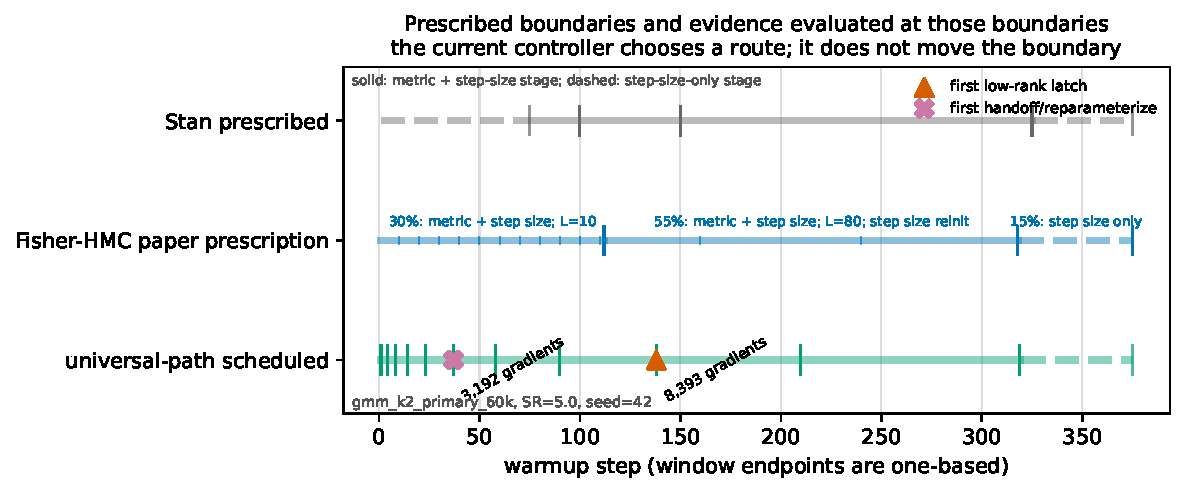
\includegraphics[width=\linewidth]{figures/schedule_evidence.pdf}
  \caption{Schedule evidence and one executed controller trace. The Stan and
  Fisher-HMC lanes are unexecuted reference prescriptions; Fisher-HMC denotes
  the specific $30/55/15$ prescription in \citet{seyboldt2026preconditioning}.
  Universal-path route decisions occur only at prescribed, unmoved boundaries:
  the scalar-gate implementation does not fit change-point timing. In the displayed
  trace the first population-handoff marker is transient and clears; terminal
  global exploration remains \texttt{not\_established}.}
  \label{fig:schedule}
\end{figure}

\paragraph{Full factorial.}
The validated schedule-by-buffer experiment reveals a severe failure on radon
for the \emph{bundle} combining proportional-growing windows with an
accumulating/per-draw-recompute buffer. Because accumulation and recomputation
move together in this arm, the result does not identify accumulation alone as
the cause. The remaining cells show that schedule, buffer, and controller
semantics must be compared as configurations rather than as a pure window-shape
effect. The Universal-path boundaries in Figure~\ref{fig:schedule} are
prescribed before execution and are not moved by detected events.

\paragraph{Restart ablation.}
Continuous dual averaging has mixed efficiency: it wins $3/6$ cells, with
continuous/reseed ratios from $0.9464$ to $1.1385$ and geometric means $1.014$
for the ill-conditioned target and $1.024$ for German credit. It reduces the
recorded oscillation and warmup-divergence burden, but this limited ablation
establishes neither directional efficiency nor equivalence between Stan and
\texttt{nutpie}.

\enlargethispage{\baselineskip}
\section{Full warmup signature}\label{app:api}

\begin{lstlisting}[language=Python,basicstyle=\ttfamily\footnotesize,
                   aboveskip=2pt,belowskip=2pt]
staged_adaptation(
  algorithm, logdensity_fn, metric="welford_diag" | MetricRecipe | MetricCore,
  *, max_grad_budget=None, n_chains=1, imm_shrinkage_to_previous=0.0,
  initial_inverse_mass_matrix=None, initial_step_size=1.0,
  target_acceptance_rate=0.80, adaptation_info_fn=..., integrator=velocity_verlet,
  schedule_fn=None, initial_metric_state=None, **extra_parameters)
\end{lstlisting}
{\small Step-size dual averaging and the stage schedule live in the host;
mass-matrix estimation is delegated to \texttt{metric}.\par}

\end{document}
